\subsection{Validação}

O método de Newton utilizado para encontrar o mínimo da Equação~\ref{eq:nr-opt}, tendo o ponto mínimo $\bar{X} = (1,2)$.
Então para obter tal resultado foi empregado duas variações do método de Newton \cite{ruggiero2000calculo,quarteroni2010numerical}.
A primeira, calcula a inversa da matriz Hessiana, vide o Algoritmo~\ref{alg:inv-opt}.
Já, a segundo utiliza a decomposição LU, disponível no Algoritmo~\ref{alg:opt} em alternativa da matriz inversa, que possui um alto custo computacional para a realizar o seu cálculo.
Portanto, ao analisar os valores do tempo de execução de um método contra o outro é nítida a vantagem da decomposição LU em comparação a Matriz Inversa.
O Algoritmo~\ref{alg:inv-opt} que utiliza a Matriz Inversa~\footnote{https://github.com/sswellington/GA018/blob/main/log/newton-opt/time-n-sys-inversa.txt} possui a média  de execução de $5,774522781$ segundos e o desvio padrão de $0,4805941876$.
Finalmente, o resultado do teste aplicado aos algoritmos, em suma o teste é a média e o desvio padrão do tempo de execução dos algoritmos, no qual é repetido 100 vezes para ser obter a média sem viés ou acaso, a fim de obter o melhor método.
o Algoritmo~\ref{alg:opt} que usa a decomposição de LU~\footnote{https://github.com/sswellington/GA018/blob/main/log/newton-opt/time-n-opt-lu.txt} tem a média de execução de $0,0916364193$ segundos e o desvio padrão de $0,04318986438$.
Logo, o Método de Newton com a decomposição de LU, vide o Algoritmo~\ref{alg:opt}, é o ideal para encontrar o ponto mínimo dessa função.


\subsection{Conclusão}
O Método de Newton com decomposição LU aplicado a Equação~\ref{eq:nr-opt}, tendo a precisão de $10^{-8}$ e ponto de partida o ponto $x_{0} = (0,0)$ o resultado está disponível na Tabela~\ref{tab:opt-LU}, no qual representa todas iterações do Método de Newton com decomposição LU. 
A Figura~\ref{img:opt-LU} ilustra a evolução do processo iterativo pela Tabela~\ref{tab:opt-LU}.
Por fim a Figura~\ref{img:opt-LU-convergencia} é a análise do erro
obtido em cada iteração.
 

\begin{table}[!htp]
\caption{Método de Newton com decomposição LU - Evolução do processo iterativo}
\label{tab:opt-LU}
\begin{tabular}{|c|c|c|c|c|c|}
\hline
\textbf{Iteração} & \textbf{Eixo X} & \textbf{Eixo Y} & \textbf{Eixo X-1} & \textbf{Eixo Y-1} & \textbf{Norma da matriz} \\ \hline
1                 & 1,061376269     & 2,275142385     & 0                 & 0                 & 3,336518654              \\ \hline
2                 & 0,9741326823    & 1,880732943     & 1,061376269       & 2,275142385       & 0,4816530295             \\ \hline
3                 & 1,001522677     & 2,007197686     & 0,9741326823      & 1,880732943       & 0,1538547379             \\ \hline
4                 & 0,999999692     & 1,999998508     & 1,001522677       & 2,007197686       & 0,0087221625             \\ \hline
5                 & 1               & 2               & 0,999999692       & 1,999998508       & 0,000001799718643        \\ \hline
6                 & 1               & 2               & 1                 & 2                 & 0                        \\ \hline
\end{tabular}
\end{table}


\begin{figure}[!htp]
    \centering
    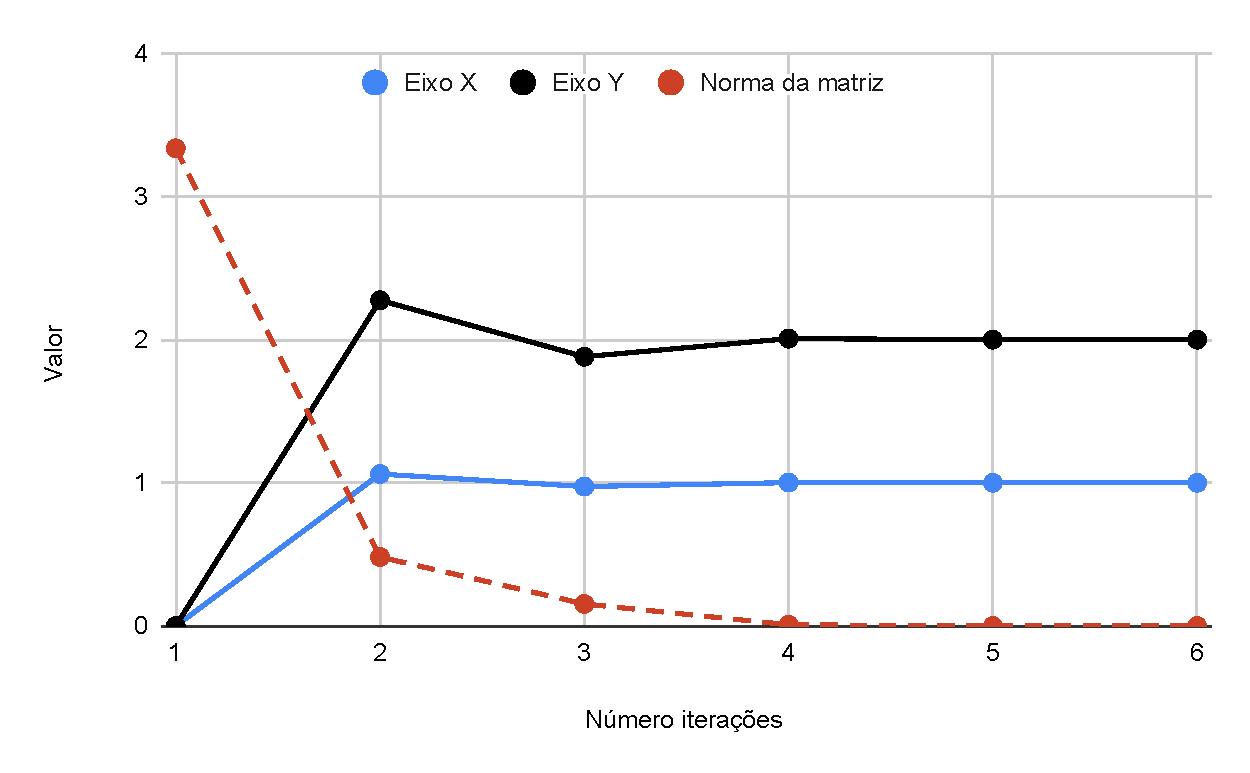
\includegraphics[scale=.7]{img/nr-opt.pdf}
    \caption{Método de Newton com decomposição LU - Evolução do processo iterativo}
    \label{img:opt-LU}
\end{figure}

\begin{figure}[!htp]
    \centering
    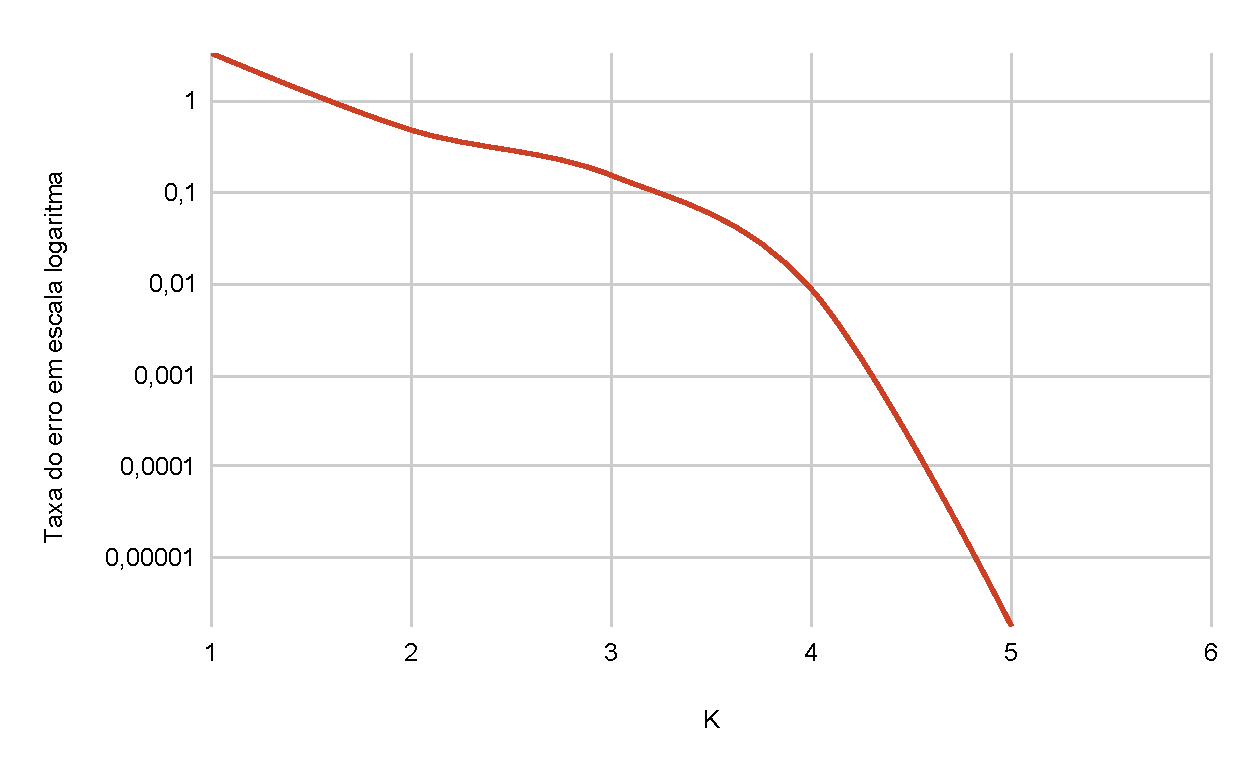
\includegraphics[scale=.7]{img/nr-opt-convergencia..pdf}
    \caption{Método de Newton com decomposição LU - Taxa de convergência obtido em cada iteração}
    \label{img:opt-LU-convergencia}
\end{figure}